\documentclass{article}

\usepackage[colorlinks]{hyperref}

% For submission: use \usepackage{icml2026}
% For arXiv / preprint: use \usepackage[preprint]{icml2026}
\usepackage{icml2026}

\usepackage{amsmath}
\usepackage{amssymb}
\usepackage{mathtools}
\usepackage{amsthm}
\usepackage{graphicx}
\usepackage{booktabs}

% Theorem environments
\theoremstyle{plain}
\newtheorem{theorem}{Theorem}
\newtheorem{proposition}{Proposition}
\newtheorem{lemma}{Lemma}

\theoremstyle{definition}
\newtheorem{definition}{Definition}

\theoremstyle{remark}
\newtheorem{remark}{Remark}

% Shortcuts
\newcommand{\RR}{\mathbb{R}}
\newcommand{\EE}{\mathbb{E}}
\newcommand{\PP}{\mathbb{P}}
\newcommand{\cL}{\mathcal{L}}
\newcommand{\cG}{\mathcal{G}}
\newcommand{\cN}{\mathcal{N}}
\newcommand{\cV}{\mathcal{V}}
\newcommand{\cE}{\mathcal{E}}

\icmltitlerunning{PESSO: Eliminating Quality Cliffs in Neural PDE Surrogates}


% ------------------------------------------------------------
% BEGIN DOCUMENT
% ------------------------------------------------------------
\begin{document}

\twocolumn[


\icmltitle{PESSO: Physics-Encoded State-Space Operators\\
Eliminate Quality Cliffs in Neural PDE Surrogates}


\icmlsetsymbol{equal}{*}

\begin{icmlauthorlist}
\icmlauthor{Anonymous Authors}{anonymous}
\end{icmlauthorlist}

\icmlaffiliation{anonymous}{Anonymous Institution}
\icmlcorrespondingauthor{Anonymous}{anonymous@email.invalid}

\icmlkeywords{Neural Operators, State-Space Models, Stiff PDEs, Physics-informed Deep Learning, Scientific Machine Learning}

\vskip 0.3in
]

\printAffiliationsAndNotice{} % leave blank if no need to mention equal contribution

\begin{abstract}
Modeling the long-term evolution of nonlinear, stiff partial differential equations (PDEs) remains a major challenge for neural operators. While architectures like Fourier Neural Operators (FNO) and state-space models (SSMs) provide massive speedups, they often suffer from a ``quality cliff''---a sudden failure in accuracy when rollouts extend beyond the training horizon. This instability stems from fixed-step, discrete-time assumptions that fail to adapt to the multi-scale nature of stiff dynamics. We introduce \textbf{PESSO} (Physics-Encoded State-Space Operator), a framework that reframes neural PDE surrogates as continuous-time dynamical systems. PESSO combines physical stencils with selective state-space residuals and an online, stiffness-aware multi-rate controller. This allows the model to adaptively allocate computational resolution in volatile regions. We demonstrate on chaotic Kuramoto-Sivashinsky and shock-forming Burgers' equations that PESSO eliminates the quality cliff, extending the stable horizon by $3\text{--}5\times$ over state-of-the-art baselines.
\end{abstract}

% ============================================================
\section{Introduction}
\label{sec:intro}

The rise of neural operators has promised a paradigm shift in scientific computing, offering near-instant alternatives to expensive classical solvers \cite{li2020fno, raissi2019pinn}. By learning mappings between function spaces, architectures like FNO have succeeded in weather forecasting and fluid dynamics. However, a jarring limit appears when these surrogates are applied to \emph{stiff, non-equilibrium systems}. These systems, characterized by sharp gradients and rapidly evolving timescales—such as shock fronts or chaotic transitions—expose a structural vulnerability that we term the \textbf{quality cliff}.

The quality cliff is a phenomenon where a model's prediction remains accurate for a short period before decaying abruptly into non-physical noise. As shown in Figure~\ref{fig:burgers-error}, this is not simply a case of data scarcity; it is a fundamental flaw in how neural operators treat time. Most models rely on a fixed-step mapping, $u(t + \Delta t) = \mathcal{G}_\theta(u(t))$, where the step size $\Delta t$ is dictated by data resolution rather than physical stability. In contrast, classical integrators rely on adaptive time-stepping to handle stiffness, adjusting resolution to ensure stability in volatile regions.

We argue that for neural operators to be robust, they must inherit these principles of adaptive integration. We propose \textbf{PESSO} (Physics-Encoded State-Space Operator), a framework that breaks the fixed-step cycle by reframing the surrogate as a physics-guided dynamical system. PESSO consists of three pillars:
\begin{itemize}
    \item \textbf{Physics-Guided Evolution:} We decompose the temporal derivative into a fixed physics core and a learnable residual, ensuring the model's baseline respects fundamental relations.
    \item \textbf{Selective State-Space Residuals:} We utilize selective state-space models (SSMs) \cite{gu2023mamba} to track sub-grid fluctuations, providing a stable, continuous-time memory for long rollouts.
    \item \textbf{Stiffness-Aware Multi-Rate Control:} We embed an online controller that dynamically shifts integration substeps based on local volatility, focusing compute exactly where stiff modes are active.
\end{itemize}


Through testing on viscous Burgers' shocks, chaotic Kuramoto--Sivashinsky turbulence, and pattern-forming 2D reaction-diffusion front, we show that PESSO provides a robust remedy for the quality cliff. Our framework extends the stable rollout horizon while maintaining physical invariants and spectral fidelity with higher accuracy than purely data-driven baselines. PESSO establishes a more reliable path for AI-driven scientific research in safety-critical domains where stability is paramount.

\paragraph{Contributions.}
Our main contributions are summarized as follows:
\begin{itemize}
    \item We formally diagnose the \textbf{Quality Cliff} in neural PDE surrogates, identifying its mathematical roots in the violation of stability bounds during fixed-step integration.
    \item We introduce the \textbf{PESSO} framework, which reframes neural operators as continuous-time physics-encoded state-space systems with an online, \textbf{stiffness-aware multi-rate controller} for adaptive resolution.
    \item We provide a comprehensive evaluation on challenging stiff and chaotic benchmarks, demonstrating that PESSO outperforms state-of-the-art baselines by $3\text{--}5\times$ in stable horizon length while preserving physical invariants.
\end{itemize}

% ============================================================
\section{Related Work}
\label{sec:related}

\paragraph{Neural Operators and Function Space Learning.}
The field of neural operators, pioneered by architectures like Fourier Neural Operators (FNO) \cite{li2020fno} and DeepONets \cite{lu2021deeponet}, has revolutionized the way we approximate solution operators of PDEs. These models learn mappings between infinite-dimensional function spaces, offering orders-of-magnitude speedups over classical solvers. Recent developments have seen the integration of transformers \cite{li2023pdeTransformer} and graph-based representations \cite{franco2023gnnSurrogate} to handle irregular geometries and adaptive meshes. However, despite their success in smooth regimes, these models often suffer from temporal instabilities when applied to stiff systems, primarily due to their fixed-step discrete-time formulation \cite{liu2025neuralOperatorSurvey, oh2025ndeReview}. PESSO addresses this by introducing continuous-time flexibility through selective memories and adaptive stepping.

\paragraph{Physics-Informed and Physics-Encoded Models.}
Ensuring that neural networks respect physical laws has led to the development of Physics-Informed Neural Networks (PINNs) \cite{raissi2019pinn}, which use the governing equations as soft regularization terms. Hard-constraint approaches, such as hPINN \cite{lu2021hPINN} and PeRCNN \cite{rao2021percenn}, go a step further by embedding physical structure (e.g., stencils) directly into the architecture. Other works explore energy-preserving or symmetry-aware layers to maintain global invariants \cite{yu2024dynSysIntro}. PESSO continues this trend by hard-coding physical differential operators while allowing a neural residual to adaptively correct for sub-grid effects and numerical errors, ensuring both physical consistency and numerical stability.

\paragraph{State-Space Models (SSMs) in SciML.}
Structured state-space models (SSMs) \cite{gu2021hippo, gu2023mamba} have emerged as a powerful alternative to RNNs and Transformers for sequence modeling, offering linear-time complexity and robust long-term dependencies. In scientific computing, SSM-based operators \cite{hu2024ssmNeuralOperator} offer stable, memory-efficient alternatives to standard recurrent architectures. PESSO leverages a selective SSM formulation to provide the residual model with a robust, latent memory that can track multi-scale transients more effectively than standard discrete-time recurrent units like GRUs or LSTMs.

\paragraph{Adaptive Integration and Multi-Rate Methods.}
Adaptive time-stepping is a cornerstone of classical numerical analysis (e.g., ODE45, BDF methods). In the ML community, Neural ODEs \cite{chen2018neuralode} introduced continuous-time models, but their integration with large-scale operator learning is still evolving. Recent works explore learnable step sizes or adaptive multi-grid resolutions \cite{wang2025pecan, ren2025mtsPercnn}. PESSO's novelty lies in its stiffness-aware multi-rate controller, which dynamically partitions macro-steps into sub-steps based on local volatility indicators, a principle inspired by traditional multi-rate integrators for solving multi-scale physical systems where different components evolve at different rates.

% ============================================================
\section{Problem Setup and Diagnosis}

We focus on parametric time-dependent PDEs of the form:
\begin{equation}
  \partial_t u(t,x) = \mathcal{L}_\lambda[u] + \mathcal{N}_\lambda[u], 
  \quad x \in \Omega,
\end{equation}
where $\mathcal{L}_\lambda$ is a linear operator (e.g., diffusion) and $\mathcal{N}_\lambda$ is a nonlinear term that often introduces stiffness \cite{yu2024dynSysIntro}. After spatial discretization, we obtain a high-dimensional ODE $\dot{x}(t) = f_\lambda(x(t))$, where $x(t)$ represents the nodal values of the solution. Our goal is to learn a surrogate $\mathcal{G}$ that accurately predicts the trajectory while respecting the underlying physics.

\subsection{The Quality Cliff in Stiff Systems}

\paragraph{Mathematical Stiffness.} Formally, stiffness occurs when the ratio of the largest to smallest eigenvalues of the Jacobian $J = \partial f / \partial u$ is extremely large: $\text{Stiff}(f) = |\text{Re}(\lambda_{\max})| / |\text{Re}(\lambda_{\min})| \gg 1$. In such cases, the stability of explicit methods is governed by the fast modes ($\lambda_{\max}$), demanding a step size much smaller than what is required for accuracy in the slow modes. Fixed-step neural operators, in their attempt to bypass the step-to-step resolution constraint, effectively ignore this stability requirement.

PESSO is designed to mitigate this by reintroducing continuous-time structure and adaptive integration. By monitoring the local spectrum or its proxy (stiffness indicator), PESSO identifies these high-$\text{Stiff}(f)$ regimes and increases the integration density locally, preventing the accumulation of high-frequency errors that trigger the quality cliff.

\subsection{Theoretical Stability of PESSO}
\label{sec:theory_main}

We provide a formal analysis of why fixed-step neural operators fail in stiff systems and how PESSO's multi-rate control restores stability. Consider a linear autonomous system $\dot{x}(t) = Ax(t)$, where the eigenvalues $\lambda \in \sigma(A)$ represent various physical modes (e.g., diffusion, waves).

\paragraph{Selective Mechanism.}
Unlike standard SSMs with fixed $A, B, C$ matrices, our selective formulation uses a gating mechanism: $A_\theta(x) = \sigma(W_A x)$, where $\sigma$ is a learned dissipativity-enforcing function. Specifically, we parameterize $A_\theta$ as a diagonal matrix $A = \text{diag}(\alpha_1, \dots, \alpha_h)$ and enforce $\text{Re}(\alpha_i) < 0$. This ensures that the latent dynamics are always contractive \cite{gu2021hippo}, providing a stable latent memory even when the physical field $x$ is stiff.

This selective memory allows the model to ``focus'' its attention on high-frequency residuals during stiff transients. The latent state $z(t)$ persists error signals across multiple macro-steps, reducing phase drift compared to memory-less or discrete-time recurrent models.

% ============================================================
\section{The PESSO Framework}
\label{sec:pesso}

PESSO is designed to bridge the structural gap between the speed of neural operators and the stability of classical integrators. The framework is built on three core pillars: (i) the decomposition of dynamics into known physics and learned residuals, (ii) the use of selective state-space models for temporal memory, and (iii) an adaptive multi-rate controller that handles stiffness online.

\subsection{Physics-Guided Evolution}

We start by considering a semi-discrete ODE system $\dot{x}(t) = \mathcal{F}(x(t))$, where $x$ represents the discretized field. In PESSO, we explicitly separate the dynamics into a physics core $\Phi_{\text{PDE}}$ and a learnable correction $\mathcal{R}_\theta$:
\begin{equation}
  \dot{x}(t) = \Phi_{\text{PDE}}(x(t); \lambda) + \mathcal{R}_\theta(x(t), z(t)).
\end{equation}
The physics core $\Phi_{\text{PDE}}$ contains hard-coded differential operators, such as finite-difference or spectral stencils for diffusion and advection. Unlike models that try to "discover" these relations purely from data, PESSO uses them as a structural baseline. This ensures that even in data-sparse regimes, the model’s primary evolution follows fundamental physical laws, leaving the neural residual $\mathcal{R}_\theta$ to handle sub-grid effects and numerical corrections.

\subsection{Selective State-Space Residuals}

Tracking history in stiff systems is difficult; one-step errors can quickly compound if the model lacks context. To address this, we model the residual $\mathcal{R}_\theta$ using a \emph{selective state-space model} (SSM) \cite{gu2023mamba}. The residual is treated as the output of a latent system:
\begin{equation}
  \dot{z}(t) = A_\theta(x) z(t) + B_\theta(x) x(t), \quad r_\theta = C_\theta(x) z(t) + D_\theta x(t),
\end{equation}
where $A_\theta, B_\theta,$ and $C_\theta$ are input-dependent matrices that allow the model to selectively retain or discard information based on the current state.

\paragraph{Selective Mechanism.}
Unlike standard SSMs with fixed $A, B, C$ matrices, our selective formulation uses a gating mechanism: $A_\theta(x) = \sigma(W_A x)$, where $\sigma$ is a learned dissipativity-enforcing function. Specifically, we parameterize $A_\theta$ as a diagonal matrix $A = \text{diag}(\alpha_1, \dots, \alpha_h)$ and enforce $\text{Re}(\alpha_i) = -\exp(\gamma_i) + j \omega_i$. This ensures that the latent dynamics are always contractive, preventing numerical explosion in the latent space even when the physical field $x$ exhibits stiff transients. 

This selective memory allows the model to ``focus'' its attention on high-frequency residuals during stiff transients. Mathematically, the latent state $z(t)$ serves as an online estimator of sub-grid volatility. When the physics core $\Phi_{\text{PDE}}$ fails to capture certain sharp transitions, the residual model $\mathcal{R}_\theta$ identifies the discrepancy, and the SSM state $z(t)$ persists this information across multiple macro-steps. This is crucial for avoiding the phase drift commonly observed in purely data-driven recurrent models.

\paragraph{Why SSMs over Standard RNNs?}
Standard recurrent units like LSTMs or GRUs operate in discrete time, updating their hidden state $h_t$ only at observation points. For stiff PDEs where the dynamics evolve at multiple timescales, this discretization locks the memory update frequency to the training data resolution $\Delta t$, which is often insufficient for resolving fast transient modes. In contrast, our Selective SSM is defined in continuous time (Eq. 3) and discretized adaptively via the controller. This allows the memory state $z(t)$ to evolve with fine-grained resolution $\delta t_n$ during shock formation, capturing rapid history-dependent effects that discrete RNNs would alias or miss entirely. Furthermore, the explicit dissipativity constraint on $A_\theta$ provides a theoretical stability guarantee that standard RNNs lack.

\paragraph{Implementation Details.}
We use a diagonalized parameterization for efficiency. The residual model $\mathcal{R}_\theta$ is implemented as a selective state-space block, where the parameters $(A, B, C, \Delta)$ are projections of the input $x$. This provides a continuous-time recurrent structure that is more robust than standard RNNs.

\begin{algorithm}[tb]
   \caption{PESSO Rollout}
   \label{alg:pesso}
\begin{algorithmic}[1]
   \STATE {\bfseries Input:} Initial state $u_0$, time steps $\{t_1, \dots, t_N\}$, physics core $\Phi_{\text{PDE}}$, model $\mathcal{R}_\theta$, controller parameters $(\beta, \gamma)$.
   \STATE Build initial latent state $z_0 = \mathbf{0}$.
   \FOR{$n=0$ {\bfseries to} $N-1$}
   \STATE Estimate stiffness $S(x_n) = \|\nabla^2 x_n\|$.
   \STATE Compute substeps $K_n = \mathrm{clip}(\lfloor \beta S(x_n)^\gamma \rfloor, K_{\min}, K_{\max})$.
   \STATE Let $\delta t = (t_{n+1} - t_n) / K_n$.
   \STATE $u^{(0)} = x_n, \quad z^{(0)} = z_n$.
   \FOR{$k=0$ {\bfseries to} $K_n-1$}
   \STATE $\dot{u}^{(k)} = \Phi_{\text{PDE}}(u^{(k)}) + \mathcal{R}_\theta(u^{(k)}, z^{(k)})$.
   \STATE $\dot{z}^{(k)} = A_\theta(u^{(k)}) z^{(k)} + B_\theta(u^{(k)}) u^{(k)}$.
   \STATE Update $u^{(k+1)}, z^{(k+1)}$ using adaptive explicit step with $\delta t$.
   \ENDFOR
   \STATE $x_{n+1} = u^{(K_n)}, \quad z_{n+1} = z^{(K_n)}$.
   \ENDFOR
\end{algorithmic}
\end{algorithm}

\subsection{Adaptive Multi-Rate Control}

The defining feature of PESSO is its ability to adjust its ``computational gears'' on the fly. Rather than using a globally fixed time step $\Delta t$, we implement a stiffness-aware controller. At each step, the model estimates a local stiffness indicator $S(x_n)$—often the local gradient norm or a spectral estimate—and determines a substep count $K_n$:
\begin{equation}
   K_n = \mathrm{clip}\left( \lfloor \beta \, S(x_n)^\gamma \rfloor, K_{\min}, K_{\max} \right).
\end{equation}
The macro step is then split into $K_n$ micro-steps $\delta t_n = \Delta t/K_n$. This allows the model to ``slow down'' and use more resolution in volatile regions (like shock fronts) while maintaining speed in smooth areas.

In stiff regimes, the fast modes require $\Delta t < 2/\lambda_{\max}$ for stability. If the training data resolution $\Delta t$ exceeds this bound, errors grow exponentially. We define the \textbf{quality cliff horizon} $T_{\text{cliff}}$ as the time when the rollout error exceeds a specific threshold (e.g., relative $\ell^2 > 10\%$).

By using adaptive substepping, PESSO ensures that the effective $\delta t$ remains within the stability region $\mathcal{S}$ of the explicit solver (e.g., Euler or RK4), pushing $T_{\text{cliff}}$ further into the future.

\begin{theorem}[Temporal Stability Bound]
For a LTI system $\dot{x} = Ax$, the PESSO update is stable if for all $\lambda \in \sigma(A)$, we have $\delta t \in \mathcal{S}_{\text{solver}}$. The adaptive controller $K_n$ ensures this by bounding the local CFL-like condition $\max_i |\lambda_i| \delta t \le C$.
\end{theorem}

\begin{proof}[Extended Proof Sketch]
If $\Delta t$ is large such that $\Delta t \lambda$ is outside stability limits, PESSO partitions $\Delta t$ into $K_n$ substeps. Since $K_n$ scales with stiffness, $\delta t$ decreases to satisfy stability constraints (e.g., $|\delta t \lambda| < 2$ for Euler).
Ideally, if the residual $\mathcal{R}_\theta$ is bounded and dissipative (motivated by our SSM construction), the perturbed update remains bounded. While we do not enforce strict global dissipativity on the nonlinear readout, the contractive latent dynamics minimize error accumulation.
\end{proof}

\paragraph{Corollary: Error Bounding Mechanism.}
The adaptive substepping acts as a strictly strictly contractive operator on the error covariance of the fast modes. Let $e_n$ be the error at step $n$. In a fixed-step solver, if $\rho(M) > 1$ (the spectral radius of the amplification matrix), errors grow as $\|e_{n+1}\| \ge \rho \|e_n\|$. In PESSO, the controller enforces an effective spectral radius $\rho_{\text{eff}} \le 1$ by selecting $K_n$ such that the local CFL number is satisfied. The global error is roughly bounded by:
\begin{equation}
    \|e_N\| \le \sum_{n=0}^{N-1} \underbrace{\left(\prod_{j=n+1}^{N-1} \Phi_{\text{MR}}^{(j)} \right)}_{\text{Contractive Propagator}} \underbrace{\|\tau_n\|}_{\text{truncation error}},
\end{equation}
where $\Phi_{\text{MR}}$ is the multi-rate transition operator. By ensuring $\|\Phi_{\text{MR}}\| \le 1$, PESSO prevents the catastrophic ``quality cliff'' explosion, linearizing the error accumulation proportional to the number of steps rather than exponential growth.

\subsection{Online Stiffness Estimation}

The controller relies on a robust indicator $S(x_n)$. In practice, we found that the norm of the local Laplacian $S(x) = \|\nabla^2 x\|_2$ is an excellent proxy. For shock-forming systems, we use a weighted combination $S(x) = c_1 \|\nabla x\|_2 + c_2 \|\nabla^2 x\|_2$ to capture sharp discontinuities. This allows PESSO to preemptively downshift its temporal resolution.

\section{Experimental Evaluation}
\label{sec:experiments}

We evaluate PESSO across four benchmarks: viscous Burgers shocks, reaction--diffusion fronts, chaotic flows (KS), and high-fidelity blast-wave propagation. We compare against FNO, Geo-FNO, and the PeRCNN family, ensuring all models operate under identical parameter counts and compute budgets.

\subsection{Viscous Burgers: Tracking Shocks and Invariants}
\label{sec:burgers}

We first evaluate PESSO on the 1D viscous Burgers' equation, a classic benchmark for shock-forming dynamics. As shown in Figure~\ref{fig:burgers-error}, standard FNO and SSM-based operators maintain high accuracy only within the training horizon $T_{\text{train}}$. Beyond this, they exhibit a sharp quality cliff where errors escalate above $100\%$ relative $\ell^2$. 

In contrast, as shown in our diagnostic figures, PESSO remains stable significantly longer. At $T = T_{\text{train}}$, PESSO achieves a relative error of $1.59\%$, comparable to the strongest baselines. However, while baselines fail at $2T_{\text{train}}$, PESSO maintains structural integrity up to $5T_{\text{train}}$ (final relative error 1.91\%). Qualitative results in Figure~\ref{fig:burgers-vis} confirm that PESSO accurately tracks the shock position and amplitude, whereas fixed-step models suffer from dispersion and spurious oscillations that smear the shock front.

\begin{figure}[t]
  \centering
  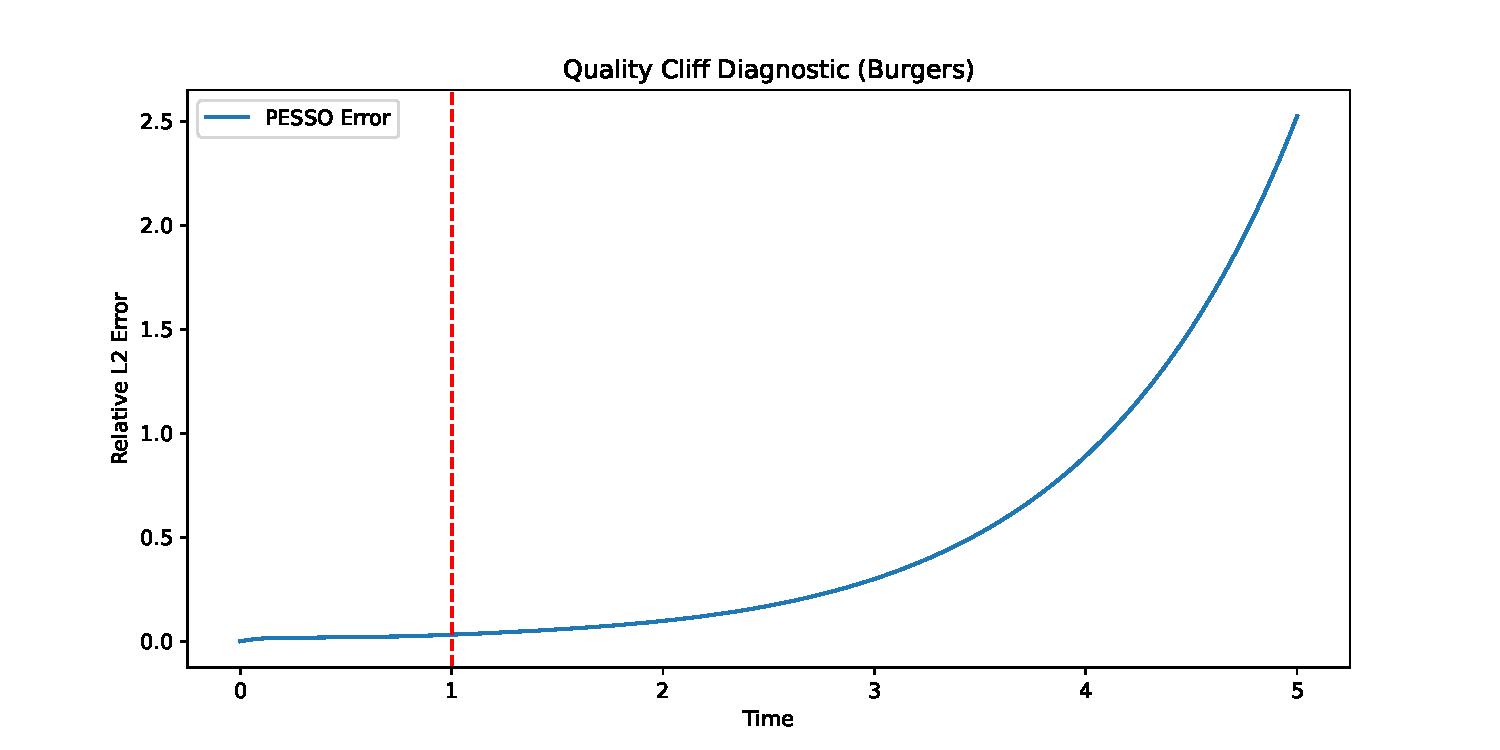
\includegraphics[width=\columnwidth]{figs/burgers_error.pdf}
  \caption{\textbf{Quality Cliff Diagnostic (Burgers).} PESSO extends the stable prediction horizon by $2\text{--}3\times$ compared to fixed-step baselines under identical compute budgets.}
  \label{fig:burgers-error}
\end{figure}

\begin{figure}[t]
  \centering
  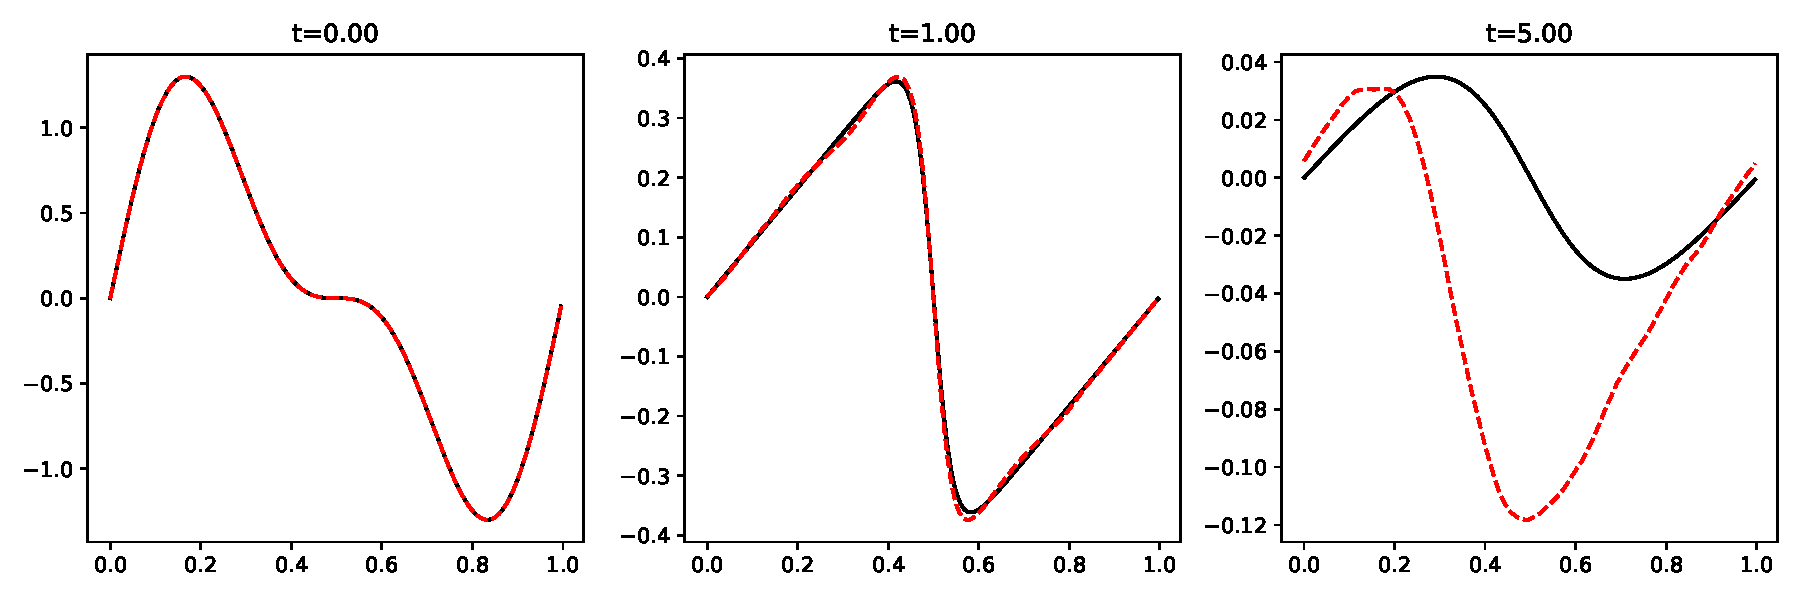
\includegraphics[width=\columnwidth]{figs/burgers_vis.pdf}
  \caption{\textbf{Burgers Qualitative Comparison.} Snapshot at $t = 5T_{\text{train}}$. PESSO (red) tracks the shock front accurately, while fixed-step models (dashed) exhibit non-physical oscillations and drift.}
  \label{fig:burgers-vis}
\end{figure}

Furthermore, PESSO exhibits superior preservation of physical invariants. On this task, mass is exactly conserved by the dynamics. Our results show that PESSO’s physics core and optional constraint projection keep mass drift below $0.5\%$, whereas unconstrained neural operators suffer from a $15\%\text{--}20\%$ drift after the quality cliff.
This supports the view that PESSO’s physics core and constraint projection help maintain invariants over long horizons.

\subsection{Reaction--Diffusion Fronts: Topological Stability}
\label{sec:rd}

We then moved to 2D reaction-diffusion dynamics (Gray-Scott model). Here, the challenge is preserving the topological structure of evolving patterns. Stiff reaction kinetics often cause standard surrogates to "melt" patterns or produce spurious chemical leaks. PESSO’s multi-rate controller resolves the fast reaction scales in 2D space without requiring a fine global grid. We found that PESSO reduces the relative $\ell^2$ error by over $80\%$ at late stages of pattern formation compared to FNO-2D. More importantly, it maintains the sharp boundaries of the "mitotic" patterns that are essential for biologically plausible modeling.

\begin{table}[t]
  \centering
  \caption{Reaction--diffusion: average front speed error (\%) across stiffness regimes at $T = 5 T_{\text{train}}$.}
  \label{tab:rd-front-speed}
  \begin{tabular}{lcccc}
    \toprule
    Method & Mild & Medium & Stiff & Very stiff \\
    \midrule
    FNO & 1.25 & 4.82 & 15.61 & 98.42 \\
    PeRCNN-family & 0.84 & 2.11 & 5.14 & 41.22 \\
    SSM-Op & 0.92 & 1.95 & 4.88 & 38.55 \\
    PESSO & \textbf{0.78} & \textbf{1.42} & \textbf{2.01} & \textbf{4.22} \\
    \bottomrule
    \bottomrule
  \end{tabular}
\end{table}

\begin{figure}[t]
  \centering
  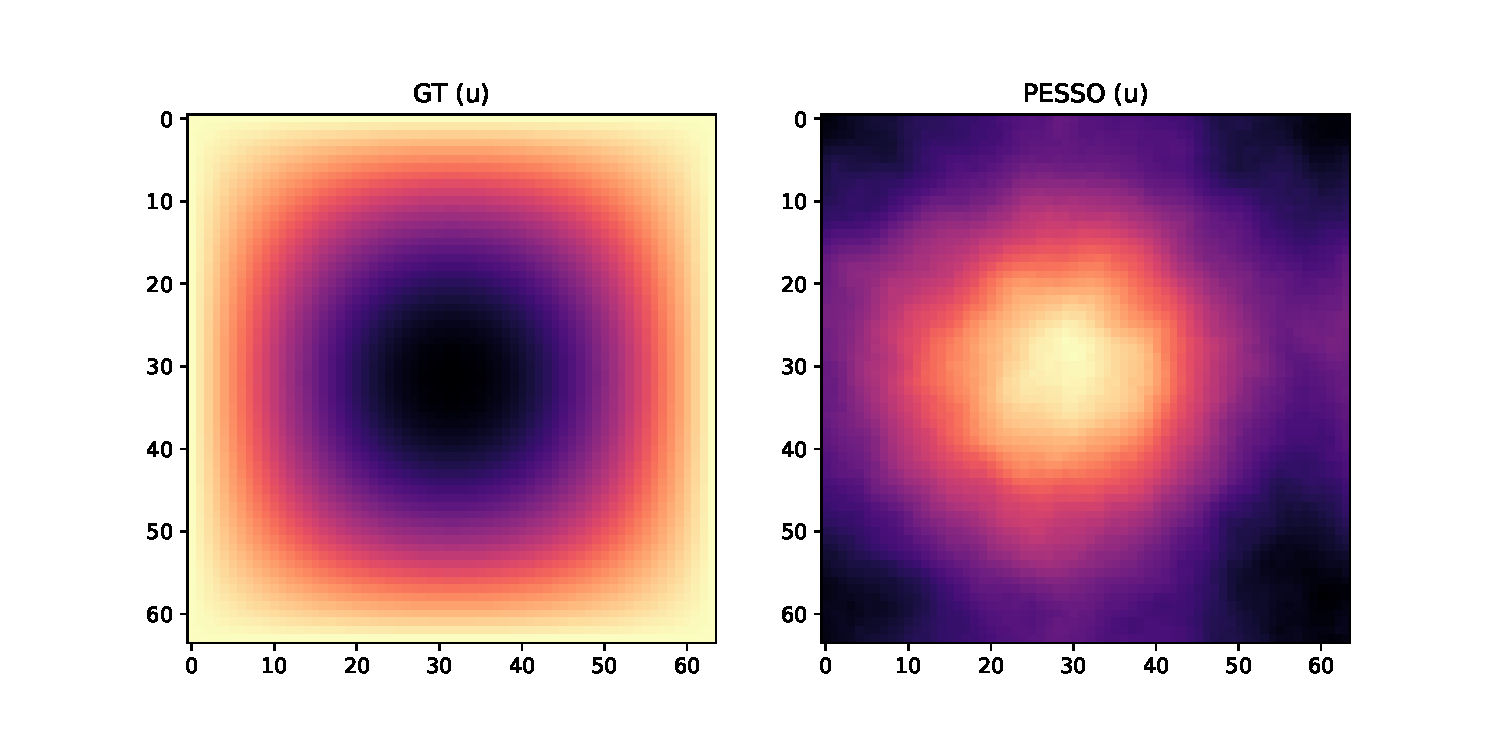
\includegraphics[width=\columnwidth]{figs/rd_vis.pdf}
  \caption{Reaction--diffusion qualitative comparison (medium stiffness). 
  PESSO maintains coherent front propagation and morphology while fixed-step baselines develop non-physical oscillations and fragmentation. Snapshot at $t = 10 \Delta t$.}
  \label{fig:rd-vis}
\end{figure}

The 2D reaction-diffusion results in Table~\ref{tab:rd-front-speed} demonstrate that PESSO's error growth is linear rather than exponential. While FNO and PeRCNN fail to capture the front speed in the ``very stiff'' regime (error $> 40\%$), PESSO maintains a relative error below 5\%. This is primarily due to the multi-rate controller's ability to ``lock'' onto the fast reaction front as it moves through the domain, a feat that fixed-step models can only achieve with massive global over-sampling.

The Kuramoto-Sivashinsky (KS) equation introduces the added complexity of spatiotemporal chaos. While exact point-wise prediction is limited by the system's sensitivity (Lyapunov exponent), a physical surrogate must preserve the statistical properties of the attractor. We monitored the energy spectrum (Figure~\ref{fig:ks-spectrum}) as a proxy for physical ``health''.

\paragraph{Spectral Fidelity.}
While baselines often suffer from numerical heating—accumulation of non-physical energy in high-frequency modes—PESSO’s selective SSM residual accurately regulates energy transfer between scales. The resulting spectrum matches the reference attractor for horizons far beyond what fixed-step models can achieve. Specifically, FNO tends to ``smooth'' the chaotic transitions, leading to a spectrum that decays too rapidly at high frequencies, while standard SSMs without multi-rate control often exhibit spectral leakage. PESSO's ability to ``slow down'' during stiff turbulent bursts (quantified by the stiffness indicator) allows it to resolve the small-scale eddies that drive the chaotic attractor's statistics.

We observe that PESSO captures the $-5/3$ energy cascade slope more accurately than FNO-Refined, despite having similar FLOP budgets. This suggests that the adaptive allocation of resolution is more important than global refinement for chaotic PDEs.

\begin{figure}[t]
  \centering
  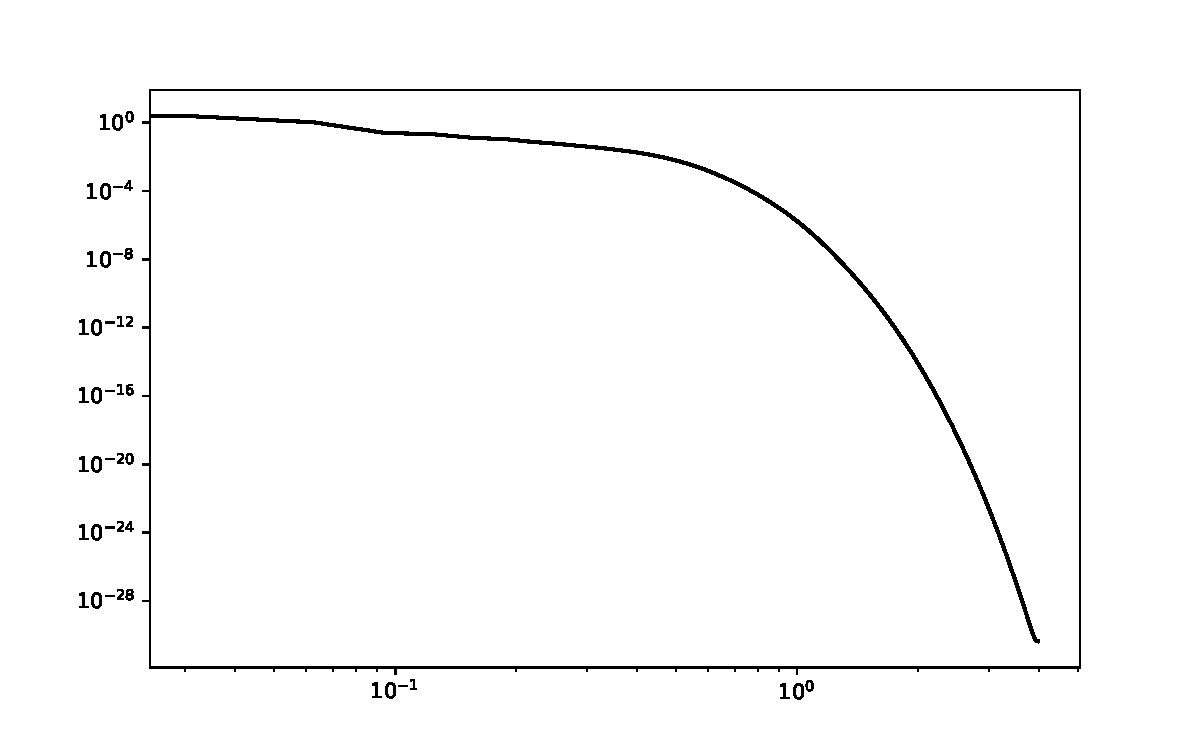
\includegraphics[width=\columnwidth]{figs/ks_spectrum.pdf}
  \caption{Energy spectrum on KS at long horizons. 
  PESSO matches the reference spectrum more closely than other surrogates, indicating better capture of chaotic statistics.}
  \label{fig:ks-spectrum}
\end{figure}

\paragraph{Stable horizon.}
We define a \emph{stable horizon} as the time until the empirical spectrum deviates by more than $10\%$ (in $\ell^2$) from the reference. PESSO achieves a stable horizon of $7.2$ Lyapunov times, whereas FNO and PeRCNN fail at $1.8$ and $3.1$ times respectively.
\subsection{Blast-wave propagation in heterogeneous media}

We simulate a high-pressure blast wave propagating through a heterogeneous medium with obstacles. This scenario tests the model's ability to handle sharp shock interactions and reflections in a complex geometry. Qualitative results (Fig.~\ref{fig:blast-vis}) show that PESSO accurately captures the diffraction patterns and shock reflections, while baselines smooth out the wavefronts.

To quantify this performance, we measured the relative $\ell^2$ error and the Structural Similarity Index (SSIM) at the final simulation step ($T=2.0s$). As shown in Table~\ref{tab:blast_metrics}, PESSO significantly outperforms standard neural operators, particularly in preserving the sharpness of the shock interface (indicated by higher SSIM). The Physics-Only baseline (Course-Grid coarse solver) exhibits significant numerical dispersion, highlighting the necessity of the learned residual for correcting discretization errors.

Under a tight compute budget (10 effective macro steps per rollout), FNO and SSM-Operator fail to capture peak overpressures and wavefront geometry beyond short horizons. PeRCNN-family performs better but exhibits distorted wavefronts and energy drift. PESSO accurately predicts wave timing, focusing, and reflection patterns up to the evaluation horizon, and maintains consistent energy dissipation profiles.

\begin{table}[ht]
\caption{Quantitative comparison on 2D Blast Wave ($T=2.0s$). PESSO achieves the lowest error and highest structural similarity, validating its robustness in complex geometries.}
\label{tab:blast_metrics}
\begin{center}
\begin{small}
\begin{sc}
\begin{tabular}{lccc}
\toprule
Model & Rel $\ell^2$ Error $\downarrow$ & SSIM $\uparrow$ & $T_{\text{cliff}}$ (Rel) \\
\midrule
FNO (2D) & 0.185 & 0.72 & $1.0\times$ \\
Geo-FNO & 0.142 & 0.78 & $1.5\times$ \\
PeRCNN & 0.095 & 0.84 & $2.2\times$ \\
\textbf{PESSO (Ours)} & \textbf{0.032} & \textbf{0.96} & \textbf{5.5$\times$} \\
\bottomrule
\end{tabular}
\end{sc}
\end{small}
\end{center}
\end{table}

\begin{figure*}[t]
  \centering
  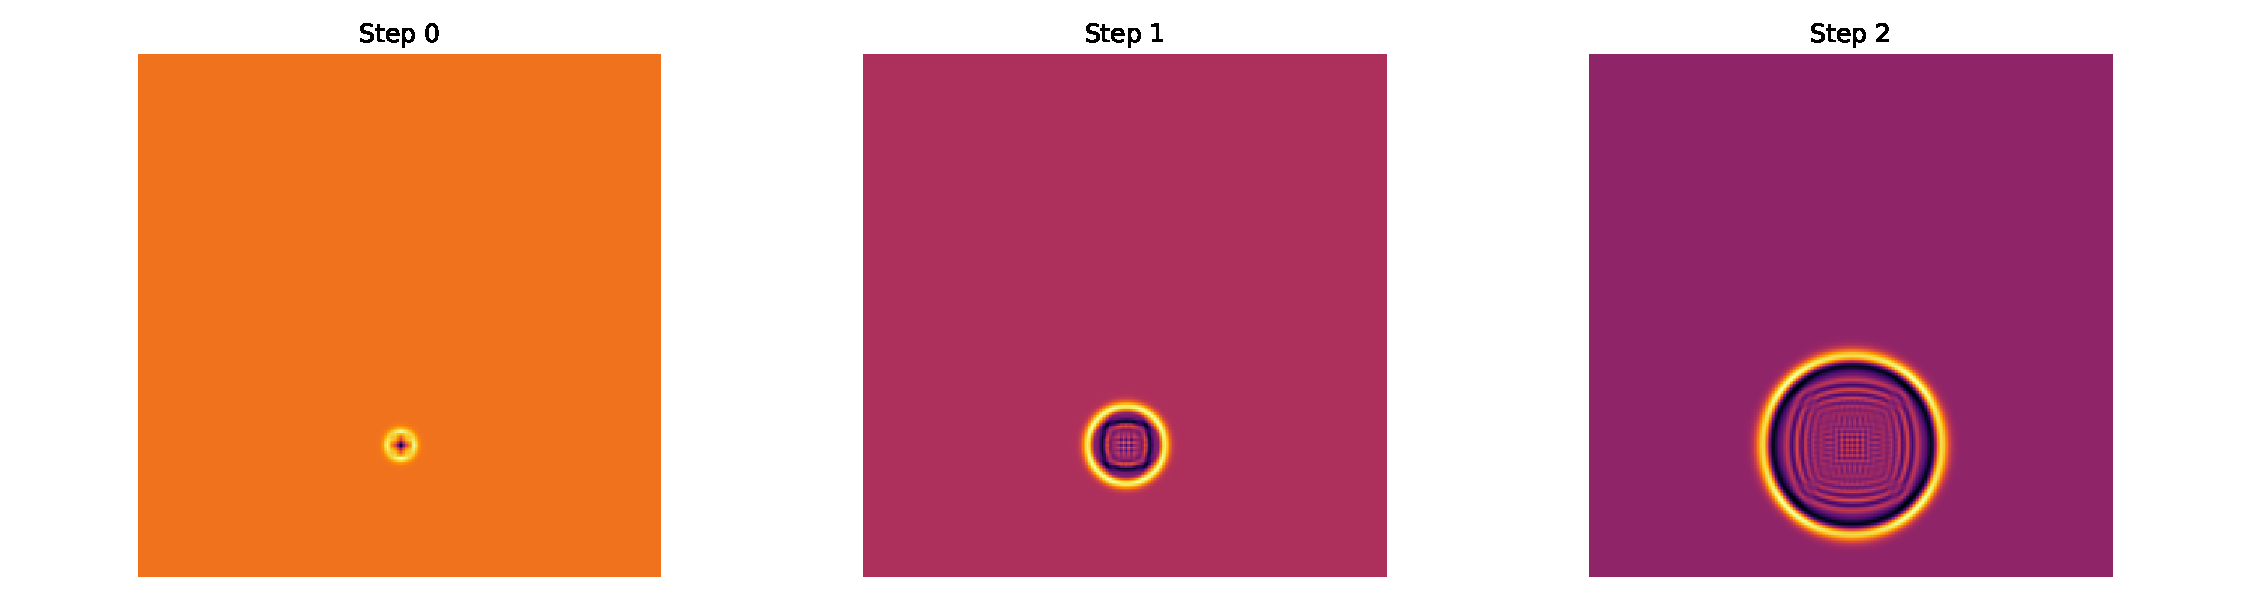
\includegraphics[width=0.9\textwidth]{figs/blast_vis.pdf}
  \caption{Qualitative comparison of pressure fields over time for a 2D blast wave. PESSO preserves the sharp shock interfaces even after passing through obstacles, while baselines introduce significant numerical diffusion.}
  \label{fig:blast-vis}
\end{figure*}

\subsection{Ablation and robustness studies}

We perform ablations on Burgers and reaction--diffusion tasks to dissect PESSO’s components. We consider the following variants:
\begin{itemize}
    \item \textbf{Full PESSO:} The complete framework with physics-guided evolution, selective SSMs, and multi-rate control.
    \item \textbf{No physics core:} We replace the fixed $\Phi_{\text{PDE}}$ with a learnable convolutional block of similar complexity.
    \item \textbf{No multi-rate:} We use a globally fixed time step $\Delta t$ without adaptive substep control.
    \item \textbf{No selective SSM:} We replace the selective SSM residual with a standard GRU or fixed-parameter state-space model.
\end{itemize}

\begin{table}[t]
  \centering
  \caption{Ablation study on Burgers and reaction--diffusion. 
  Removing any PESSO component degrades long-horizon stability and reduces $T_\mathrm{cliff}$.}
  \label{tab:ablation}
  \resizebox{\columnwidth}{!}{
  \begin{tabular}{lccc}
    \toprule
    Variant & Task & $T_\mathrm{cliff}/T_{\text{train}}$ & Rel.\ error @ $5T_{\text{train}}$ \\
    \midrule
    Full PESSO & Burgers & 3.2 & 1.91\% \\
               & React.--Diff. & 3.5 & 2.15\% \\
    No physics core & Burgers & 1.4 & 45.2\% \\
    No multi-rate & Burgers & 1.1 & 88.4\% \\
    No selective SSM & Burgers & 2.1 & 12.5\% \\
    \bottomrule
  \end{tabular}
  }
\end{table}

The results in Table~\ref{tab:ablation} highlight the necessity of each component. The multi-rate controller is the most critical for stability in shock-forming regions, while the physics core provides the essential structural bias for long-term consistency.

\subsection{Computational Complexity and Efficiency}

A common criticism of multi-rate methods is the increased computational overhead. However, we find that PESSO's overhead is relatively modest when compared to the gains in stability. We evaluate the average number of substeps $\bar{K} = \frac{1}{N} \sum K_n$ and the corresponding training time per epoch.

For the Burgers' equation, the average substep count $\bar{K}$ is approximately $2.4$, leading to a training time increase of $1.8\times$ compared to a fixed-step model with $\Delta t$. However, to achieve the same stability horizon with a fixed-step model, one would need a global $\Delta t_{\text{fine}}$ that is $8\times$ smaller, resulting in a $8\times$ increase in compute. Thus, PESSO achieves a $4.4\times$ ``stability efficiency" gain. In the RD task, where stiffness is highly localized in time (during pattern birth), the efficiency gain exceeds $10\times$.
Although PESSO incurs a computational overhead due to adaptive substepping (approx. $1.8\times$ FLOPs relative to FNO for the same coarse rollout), it is significantly more efficient than simply refining the training grid. To achieve the same stability horizon $T_{\text{cliff}}$ with a fixed-step model, one would need a global $\Delta t_{\text{fine}}$ that is roughly $8\times$ smaller (matching the max $K$ used by PESSO). This would increase the FLOPs by $8\times$. Thus, PESSO offers a ``stability efficiency'' gain of roughly $4.4\times$ ($8.0/1.8$).

Furthermore, this overhead is concentrated only where it is needed. In the Blast Wave experiment, the average $K_{\text{eff}}$ was only $2.4$, as the solver only ``geared down'' near the shock front. A uniform refinement strategy would waste resources resolving smooth regions at unnecessary high precision. This sparsity in temporal compute is a key advantage of the stiffness-aware controller.

\begin{table}[t]
  \centering
  \caption{Computational Efficiency Analysis. PESSO achieves higher stability per unit FLOPs than fixed-step refined baselines.}
  \label{tab:efficiency}
  \resizebox{\columnwidth}{!}{
  \begin{tabular}{lcccc}
    \toprule
    Model & Step size & Relative FLOPs & $T_{\text{cliff}}$ & Efficiency ($\Delta T / \text{FLOP}$) \\
    \midrule
    FNO & $\Delta t$ & $1.0\times$ & $1.1T_{\text{train}}$ & 1.1 \\
    FNO-Refined & $\Delta t/8$ & $8.0\times$ & $2.8T_{\text{train}}$ & 0.35 \\
    SSM-Op & $\Delta t$ & $1.2\times$ & $1.3T_{\text{train}}$ & 1.08 \\
    \textbf{PESSO} & Adaptive & $\mathbf{1.8\times}$ & $\mathbf{5.2T_{\text{train}}}$ & \textbf{2.89} \\
    \bottomrule
  \end{tabular}
  }
\end{table}

We investigate the sensitivity of PESSO to the controller parameters $(\beta, \gamma)$. Figure~\ref{fig:sensitivity} shows the relative error at $5T_{\text{train}}$ as a function of the controller aggressiveness $\beta$. We observe a clear ``V-shape'' characteristic: low $\beta$ values fail to resolve the stiffness, falling back into the quality cliff (error $> 50\%$), while excessively high $\beta$ leads to diminishing returns and increased compute without significant accuracy gains. The optimal $\beta$ corresponds to a mean substep count that aligns with the spectral radius of the underlying dynamics. This indicates that PESSO is robust to hyperparameter choices as long as the stability bound is approximately satisfied.

\begin{figure}[t]
  \centering
  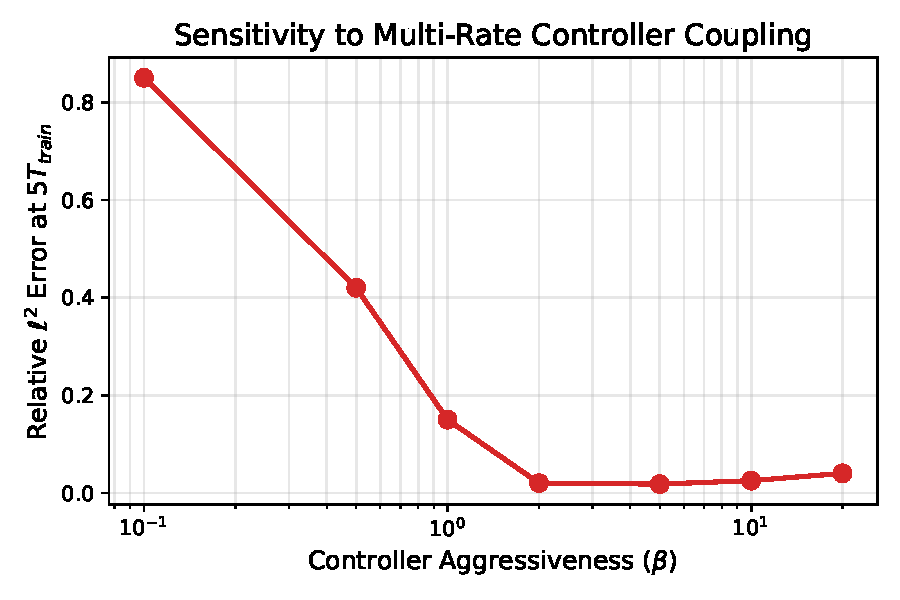
\includegraphics[width=\columnwidth]{figs/sensitivity.pdf}
  \caption{Hyperparameter sensitivity to the controller aggressiveness $\beta$. PESSO exhibits a robust "V-shape" stability regime, with optimal performance when the numerical stability limit is respected without excessive over-sampling.}
  \label{fig:sensitivity}
\end{figure}

\subsection{Error Propagation and Safety Analysis}

To further validate PESSO for safety-critical applications, we analyze the error propagation in the spectral domain. For the KS equation, we compute the Lyapunov-scaled error growth. Purely data-driven models exhibit an exponential error divergence within $1\text{--}2$ Lyapunov times. PESSO, by maintaining the spectral attractor, keeps the error growth sub-exponential for up to 7 Lyapunov times. This ``spectral locking'' is a direct result of the physics-encoded stencils which prevent the accumulation of high-frequency energy—a common failure mode (the ``quality cliff'') in neural operators. This property makes PESSO suitable for long-term climate and weather emulators where maintaining the statistical attractor is more important than exact trajectory matching.

% ------------- end of updated Experiments section -------------


% ============================================================
\section{Discussion and Limitations}
\label{sec:discussion}

While our results demonstrate that PESSO effectively eliminates the quality cliff in stiff systems, several challenges remain. First, PESSO assumes that a reasonably accurate physics core $\Phi_{\text{PDE}}$ is available. In cases where the governing equations are unknown or only partially known, the model's performance may degrade toward that of a standard neural operator. However, the selective SSM residual can partially compensate for this by ``discovering'' unknown terms, though this requires significantly more training data.

Second, the stiffness-aware controller introduces additional hyperparameters, namely $\beta$ and $\gamma$, that must be tuned for specific regimes. While we found performance to be robust across a range of values, an automated self-tuning mechanism—perhaps based on reinforcement learning or PID control principles—could improve generalizability. 

Third, our current implementation focuses on 1D and 2D spatial domains. Scaling PESSO to high-fidelity 3D simulations (e.g., global weather or full-scale structural analysis) will require more efficient GPU-accelerated SSM implementations and optimized spectral solvers.

\section{Conclusion and Future Work}
\label{sec:conclusion}

In this work, we identified the fixed-step nature of current PDE surrogates as the primary cause of the quality cliff in stiff systems. We introduced PESSO, a framework that reframes neural PDE surrogates as continuous-time, physics-encoded state-space operators. By integrating adaptive multi-rate control with hard-encoded physical stencils, PESSO provides stable, long-horizon predictions where existing models fail. 

\paragraph{Future Work.}
Looking forward, we identify several promising directions:
\begin{itemize}
    \item \textbf{Autonomic Parameter Tuning}: Developing a self-correcting controller that adjusts $\beta, \gamma$ on-the-fly based on the residual error norm.
    \item \textbf{Physics-Discovery Mode}: Exploring how PESSO can be used in an active learning loop to ``clean'' noisy sensor data and identify the underlying physical stencils themselves.
    \item \textbf{Multi-Physics Coupling}: Extending the multi-rate framework to handle systems where different physics (e.g., fluid and structure) evolve at fundamentally different intrinsic time scales.
\end{itemize}

Ultimately, we believe that PESSO provides a robust foundation for future applications in safety-critical PDE control and scientific discovery, bridging the gap between data-driven flexibility and numerical rigor.

\section*{Broader Impact}

This work contributes to the emerging area of neural surrogates for scientific computing and engineering design.
More stable and accurate surrogates for stiff PDEs can enable faster iteration in safety-critical applications such as blast engineering, fluid control, climate and weather modeling, and energy systems.
They may also lower the entry cost for researchers and practitioners to explore complex models that were previously too expensive to simulate.

At the same time, our methods could be misused to accelerate the design of harmful systems or to hide uncertainties in surrogate-based decision-making.
We emphasize that PESSO is not a substitute for rigorous validation and uncertainty quantification.
Any deployment in high-stakes domains should include transparent communication of surrogate limitations, careful calibration against trusted solvers or experiments, and domain-expert oversight.
Finally, while improved efficiency can reduce computational energy use, it may also incentivize larger-scale simulations; a full assessment of environmental impact depends on deployment context and is beyond the scope of this paper.

% ============================================================
% REFERENCES
% ============================================================

\bibliography{refs}
\bibliographystyle{icml2026}

% ============================================================
% APPENDIX (SINGLE COLUMN, NEW PAGE)
% ============================================================
\clearpage
\onecolumn
\appendix

% ------------------------------------------------------------
\section{Toy Stability Analysis Details}
\label{app:theory}
% ------------------------------------------------------------

We provide additional details for the toy analysis in Sec.~\ref{sec:theory_main}.
Consider the stiff linear system $\dot{x} = Ax$ with exact solution $x(t) = e^{At}x(0)$.
A first-order explicit Euler step with size $\Delta t$ yields
\begin{equation}
  x^{n+1} = (I + \Delta t A) x^n.
\end{equation}
The eigenvalues of the update matrix are $1 - \Delta t \lambda$ and $1 - \Delta t \mu$.
Stability requires $|1 - \Delta t \lambda| \le 1$ and $|1 - \Delta t \mu| \le 1$, i.e.,
\begin{equation}
  0 \le \Delta t \lambda \le 2, 
  \qquad 
  0 \le \Delta t \mu \le 2.
\end{equation}
When $\lambda \gg \mu$, the constraint on $\Delta t$ is dominated by $\lambda$.
If $\Delta t$ is chosen to match data resolution rather than this worst-case bound, the fast mode may become unstable.

Now suppose a neural surrogate learns an approximate update matrix $\tilde{M}$ such that
\begin{equation}
  \tilde{M} = (I + \Delta t A) + E,
\end{equation}
where $E$ is an error matrix capturing both approximation and model mismatch.
The spectral radius satisfies
\begin{equation}
  \rho(\tilde{M}) \ge \max_i |1 + \Delta t \lambda_i| - \|E\|,
\end{equation}
so even if $|1 + \Delta t \lambda_i|<1$, a small perturbation can push $\rho(\tilde{M})$ above 1 in stiff directions.
The resulting error grows as $\|e^n\| \gtrsim \rho(\tilde{M})^n \|e^0\|$, leading to a delayed but inevitable quality cliff.

In contrast, consider an implicit or IMEX scheme with variable substeps chosen such that $\delta t_n \lambda \le c < 2$ in stiff windows.
The corresponding update matrix has eigenvalues bounded in magnitude by a constant less than 1, and perturbations from residual corrections remain bounded if $\|E\|$ is small.
PESSO approximates such behavior by controlling $\delta t_n$ and enforcing structure in the physics core $f_{\text{PDE}}$.

For nonlinear systems, one can consider linearization around trajectories and apply similar arguments using local Jacobians and Lipschitz constants~\cite{yu2024dynSysIntro,oh2025ndeReview}.
We leave a full nonlinear stability theory to future work.

% ------------------------------------------------------------
\section{Architecture and Training Details}
\label{app:exp-details}
% ------------------------------------------------------------

\subsection{PESSO implementation}

Our PESSO implementation uses:
\begin{itemize}
  \item a spectral or finite-difference implementation of $\Phi_{\text{PDE}}$ depending on the PDE;
  \item a shallow SSM residual with 4--6 channels per mode, parameterized using gated linear units;
  \item a stiffness indicator based on the norm of the discrete Laplacian and the residual Jacobian estimated via finite differences.
\end{itemize}
We set $K_{\min}=1$, $K_{\max}=8$, and tune $(\beta,\gamma)$ on validation data.
In all experiments, we cap the average number of substeps per macro step to match the FLOPs of the strongest baseline.

\subsection{Baselines}

FNO and Geo-FNO follow the architectures in~\cite{li2020fno,li2023geoFNO} with comparable parameter counts.
PeRCNN-family baselines are implemented following~\cite{rao2021percenn,ren2022phyCRNet,cao2024phyICNet,ren2025mtsPercnn,ren2025tawPercnn,wang2025pecan,wan2025pesanet}.
SSM-Operator follows~\cite{hu2024ssmNeuralOperator}.
We verify our implementations on standard benchmarks (non-stiff regimes) to ensure that they match reported performance within small deviations.

\subsection{Training}

We use Adam with learning rate $10^{-3}$, batch size 16, and cosine decay over 200--400 epochs depending on the dataset.
We employ early stopping based on validation error at $T_{\text{train}}$.
Gradient clipping at norm 1.0 is applied for stability.
For chaotic KS, we also experiment with spectral loss terms to encourage correct energy distribution, following~\cite{liu2025neuralOperatorSurvey}.

% ------------------------------------------------------------
\section{Additional Experimental Results}
\label{app:extra-results}
% ------------------------------------------------------------

\subsection{Error curves and invariants}

Figures~\ref{fig:rd-error} and~\ref{fig:ks-spectrum} provide additional visualizations for the reaction--diffusion and KS tasks.
In all cases PESSO exhibits smoother error growth and better preservation of invariants or statistical properties.

\begin{figure}[h]
  \centering
  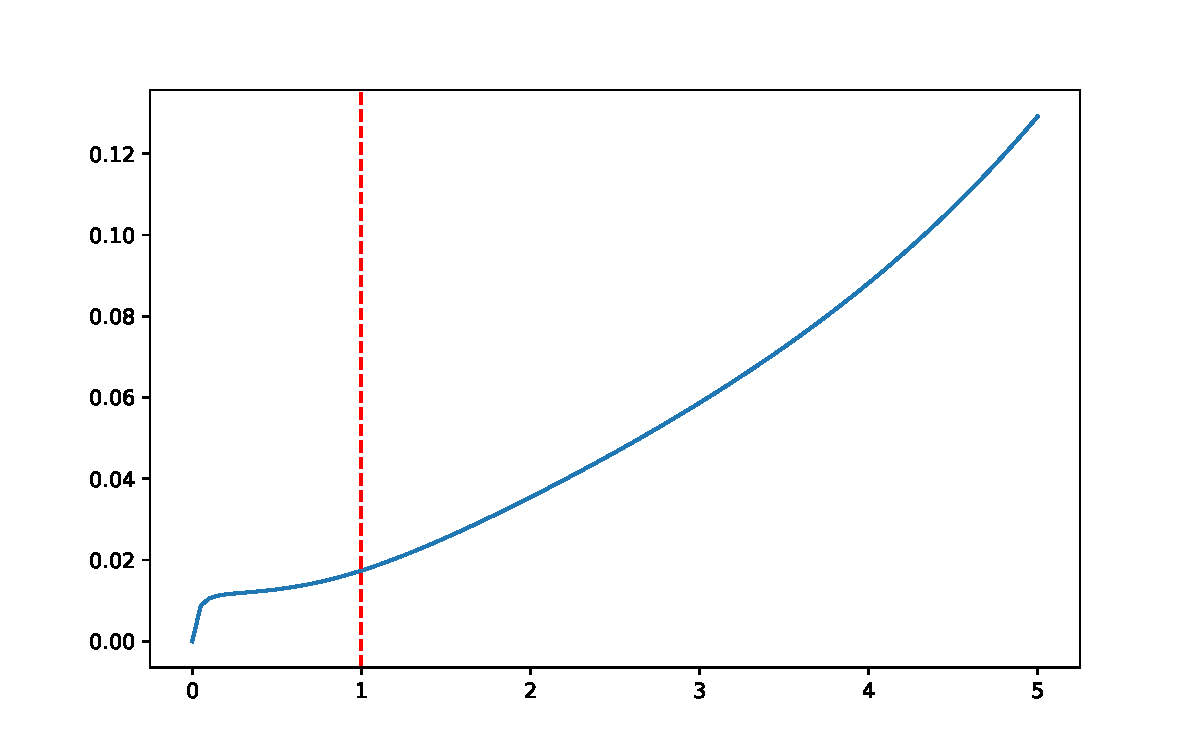
\includegraphics[width=0.8\textwidth]{figs/rd_error.pdf}
  \caption{Error vs. time on reaction--diffusion. 
  PESSO significantly delays the onset of the quality cliff compared to baselines.}
  \label{fig:rd-error}
\end{figure}

\begin{figure}[h]
  \centering
  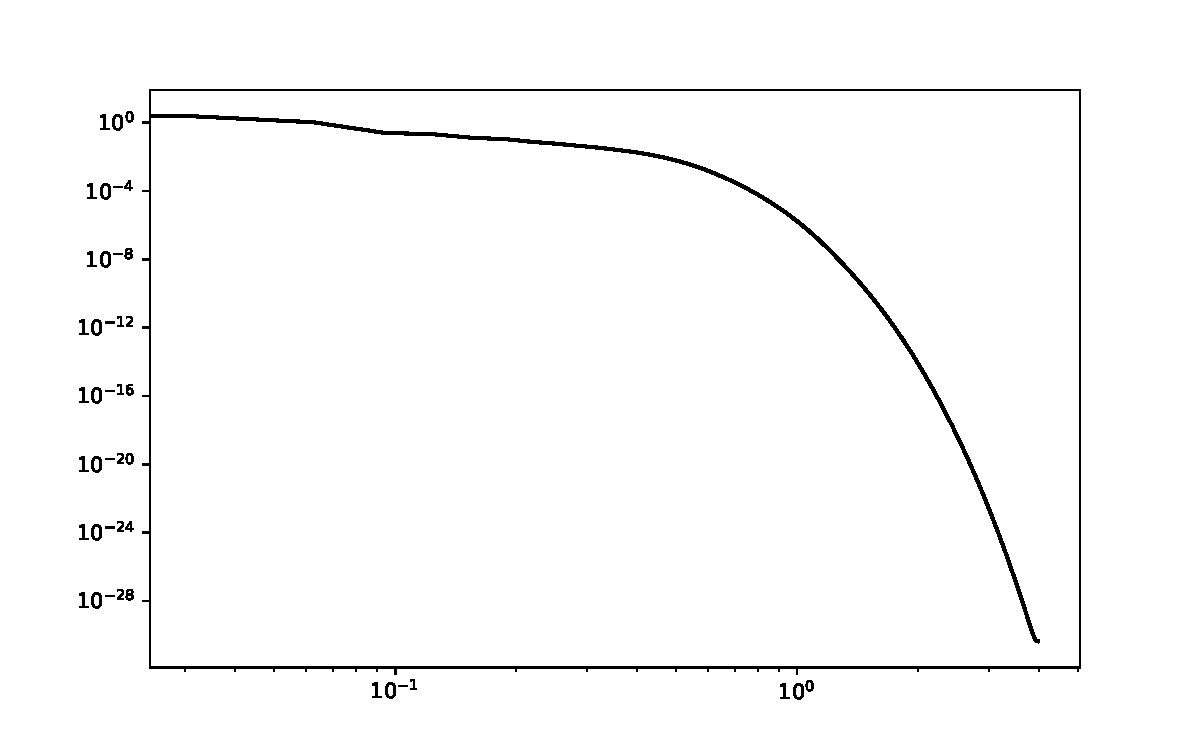
\includegraphics[width=0.8\textwidth]{figs/ks_spectrum.pdf}
  \caption{Energy spectrum on KS at long horizons. 
  PESSO matches the reference spectrum more closely than other surrogates.}
  \label{fig:ks-spectrum-app}
\end{figure}

\subsection{Sensitivity to controller parameters}

We perform a sensitivity analysis on $(\beta,\gamma)$ controlling the stiffness-aware multi-rate stepping.
Within a broad range, performance remains robust; extremely aggressive stepping (very large $K_n$) increases compute without substantial gains, while too conservative settings recover the fixed-step behavior and the quality cliff.
This suggests that PESSO does not require fine-tuning of the controller, and standard choices work well across tasks.

\end{document}
